\documentclass[../notes.tex]{subfiles}

\pagestyle{main}
\renewcommand{\chaptermark}[1]{\markboth{\chaptername\ \thechapter\ (#1)}{}}
\setcounter{chapter}{4}

\begin{document}




\chapter{???}
\section{Planar Autonomous Linear Systems}
\begin{itemize}
    \item \marginnote{10/24:}Review of vector fields.
    \item \textbf{Phase diagram}: A diagram that shows the qualitative behavior of an autonomous ordinary differential equation. \emph{Also known as} \textbf{phase portrait}.
    \begin{figure}[h!]
        \centering
        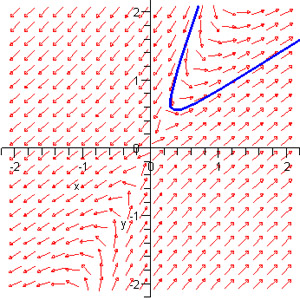
\includegraphics[width=0.4\linewidth]{../ExtFiles/exPhaseDiagram.jpeg}
        \caption{Phase diagram example.}
        \label{fig:exPhaseDiagram}
    \end{figure}
    \begin{itemize}
        \item Consists of a selection of arrows describing, to some extent, a vector field and is often paired with integral curves.
    \end{itemize}
    \item Suppose $\Omega\subset\R^n$ is open.
    \item \textbf{Vector field} (on $\Omega$): A mapping from $\Omega\to\R^n$. \emph{Denoted by} $\bm{X}$.
    \begin{itemize}
        \item Essentially, a vector field assigns to every point of some region a vector; the definition just formalizes this notion.
    \end{itemize}
    \item \textbf{Flow}: A formalization of the idea of the motion of particles in a fluid.
    \begin{itemize}
        \item The solution to the IVP $\dv{y}{t}=X(y)$, $y(0)=x$.
    \end{itemize}
    \item If $X$ is $C^1$, then for all $x\in\Omega$, there exists a unique solution $y$ to the above IVP.
    \item \textbf{Orbit} (of $x$ under $X$): The trajectory $y(t,x)$.
    \begin{itemize}
        \item Recall that the tangent vector to any trajectory at any point coincides with the vector to which $X$ maps that point.
    \end{itemize}
    \item \textbf{Fixed point}: A point $x_0\in\Omega$ such that $X(x_0)=\bar{0}$.
    \begin{itemize}
        \item If $x_0$ is a fixed point, then the trajectory is $y(t)=x_0$.
    \end{itemize}
    \item Today: We will consider flows on vector fields where the dimension is two and our vector field is linear. In particular\dots
    \item Let $A$ be a $2\times 2$ real matrix, and let $X(x)=Ax$.
    \begin{itemize}
        \item In this case, $x_0=0$ is the only fixed point.
        \item The flow is given by the linear differential equation $y'=Ay$, $y(0)=x$. The solution is $y(t)=\e[tA]x$.
    \end{itemize}
    \item Case 1: $A$ has no real eigenvalues.
    \begin{figure}[h!]
        \centering
        \begin{subfigure}[b]{0.32\linewidth}
            \centering
            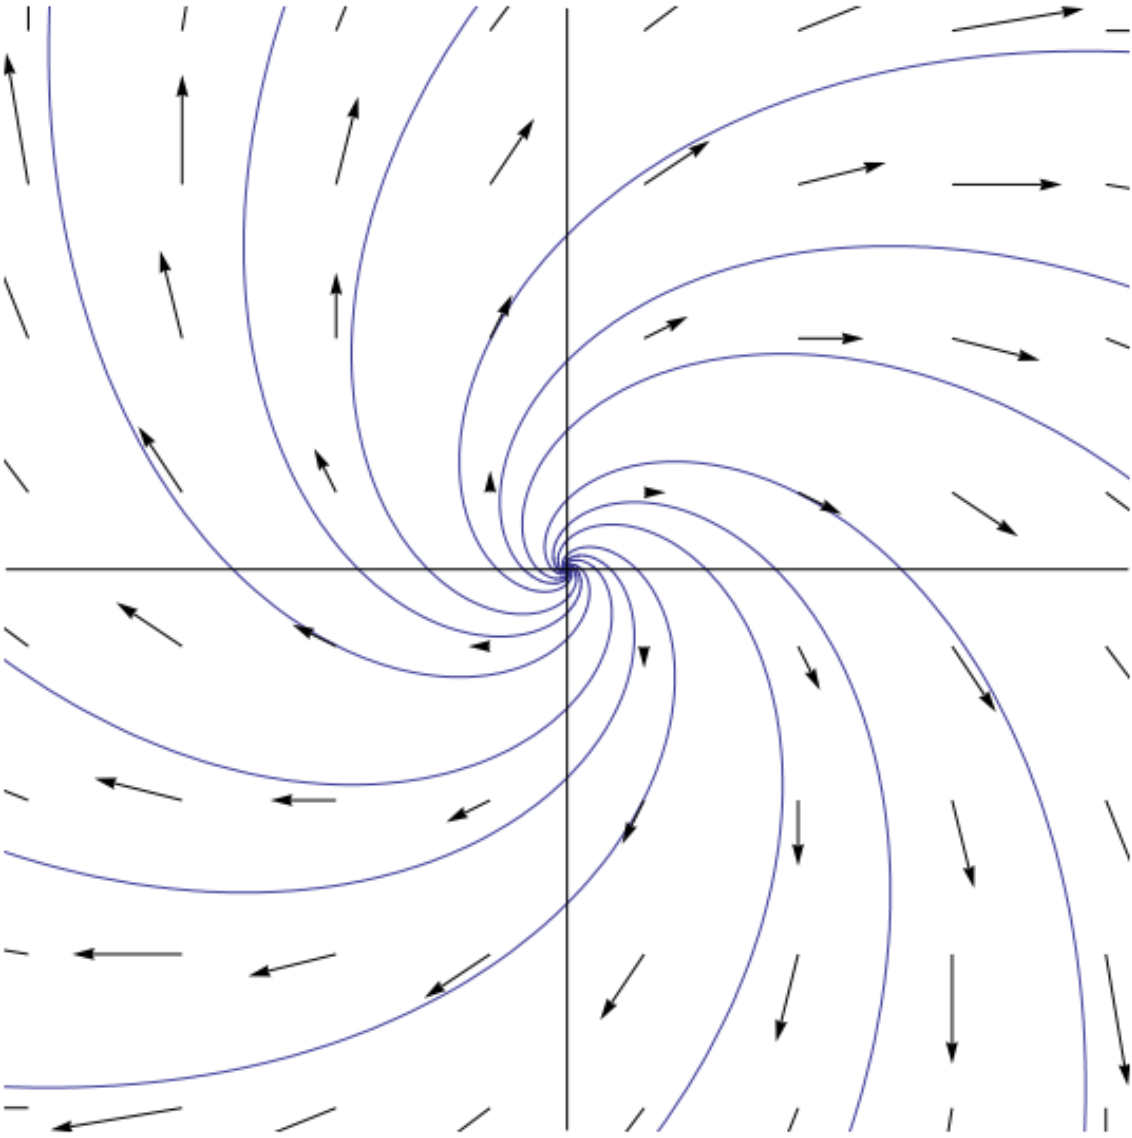
\includegraphics[width=0.8\linewidth]{../ExtFiles/planarComplexa.png}
            \caption{$\sigma>0$.}
            \label{fig:planarComplexa}
        \end{subfigure}
        \begin{subfigure}[b]{0.32\linewidth}
            \centering
            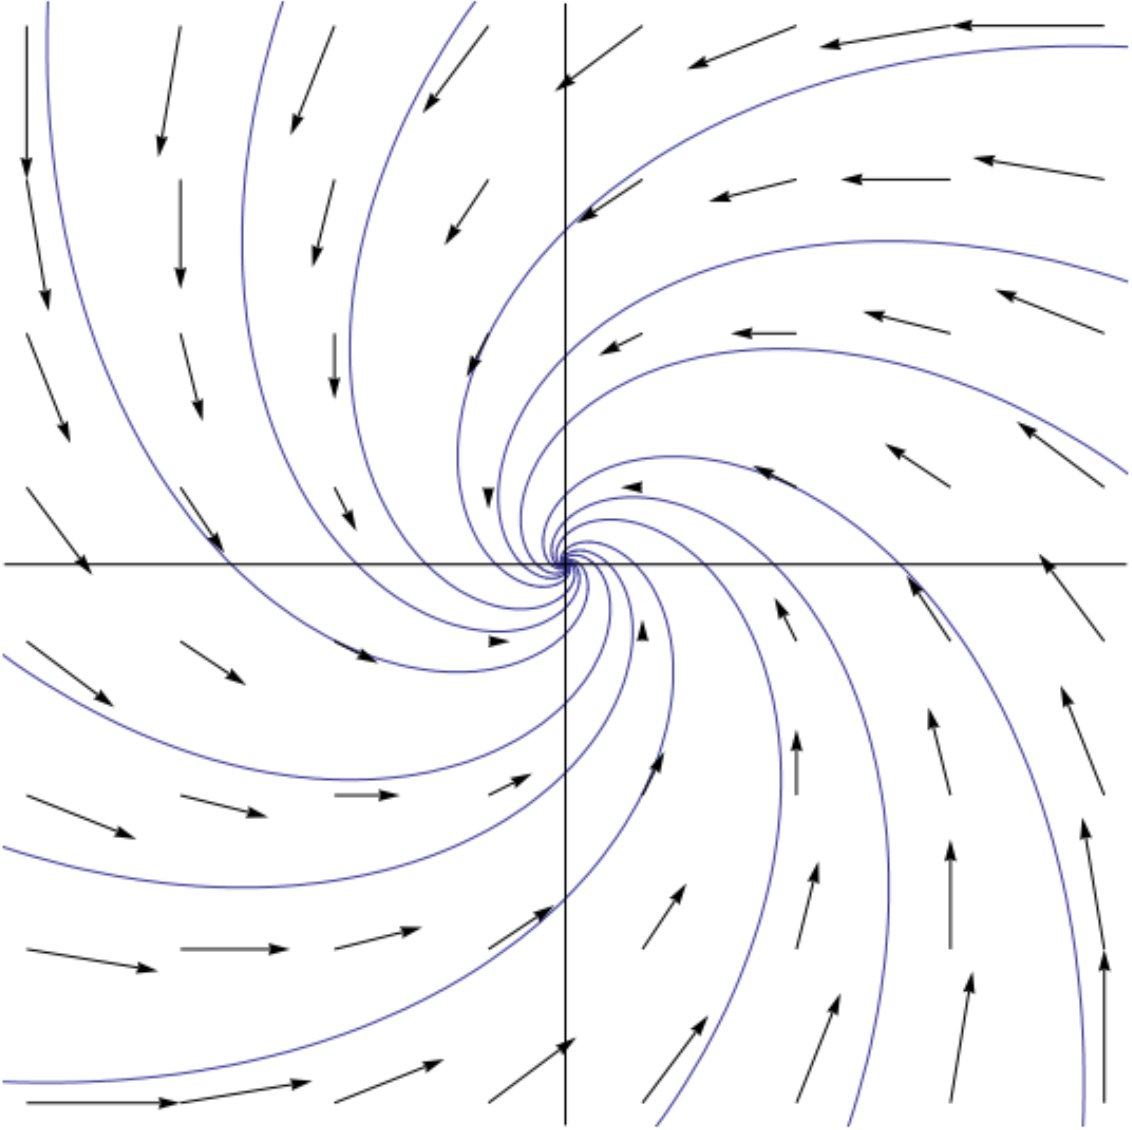
\includegraphics[width=0.8\linewidth]{../ExtFiles/planarComplexb.png}
            \caption{$\sigma<0$.}
            \label{fig:planarComplexb}
        \end{subfigure}
        \begin{subfigure}[b]{0.32\linewidth}
            \centering
            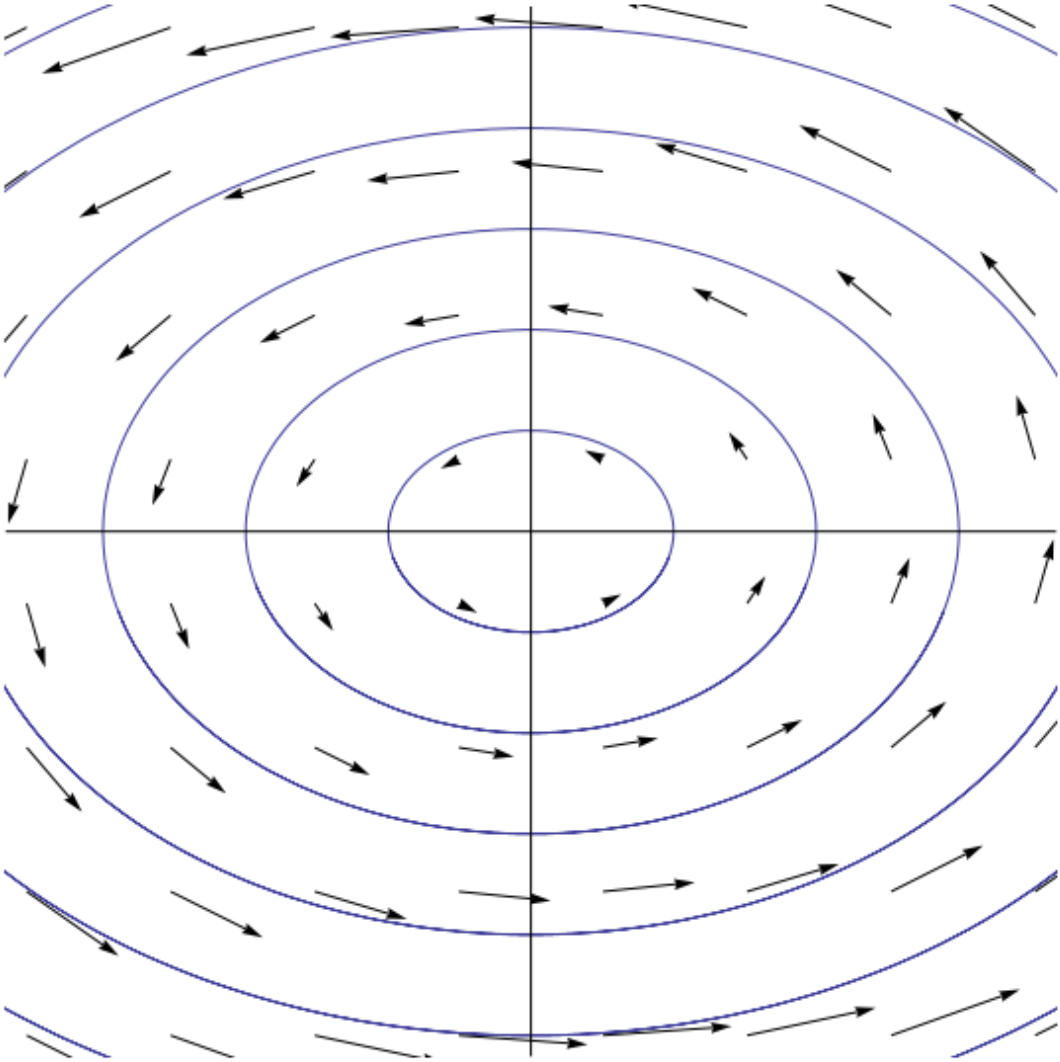
\includegraphics[width=0.8\linewidth]{../ExtFiles/planarComplexc.png}
            \caption{$\sigma=0$.}
            \label{fig:planarComplexc}
        \end{subfigure}
        \caption{Phase diagrams for a planar system with no real eigenvalues.}
        \label{fig:planarComplex}
    \end{figure}
    \begin{itemize}
        \item We know that $\chi_A(z)$ is a real polynomial: $\chi_A(z)=z^2+(\trc A)z+\det A$, and since $A$ is real, both $\trc A$ and $\det A$ are real.
        \item Thus, the eigenvalues appear as conjugate pair, i.e., we may write $\lambda=\sigma+i\beta$ and $\bar{\lambda}=\sigma-i\beta$.
        \begin{itemize}
            \item $\alpha=\gamma=1$ for both eigenvalues.
            \item The eigenvectors must also be complex conjugates.
        \end{itemize}
        \item Distinct eigenvalues imply that $A$ is diagonalizable.
        \item However, this is not what we want because if we use the complex form, then
        \begin{equation*}
            \e[tA] = Q
            \begin{pmatrix}
                \e[t\lambda] & 0\\
                0 & \e[t\bar{\lambda}]\\
            \end{pmatrix}
            Q^{-1}
        \end{equation*}
        \item Indeed, we want to get a real matrix out of $Q,\e[t\Lambda],Q^{-1}$ all complex. We have
        \begin{align*}
            \e[tA]x &= Q
            \begin{pmatrix}
                \e[t(\sigma+i\beta)] & 0\\
                0 & \e[t(\sigma-i\beta)]\\
            \end{pmatrix}
            \underbrace{Q^{-1}x}_z\\
            &= Q
            \begin{pmatrix}
                \e[t(\sigma+i\beta)]z^1\\
                \e[t(\sigma-i\beta)]z^2\\
            \end{pmatrix}\\
            &= z^1\e[t(\sigma+i\beta)]v+z^2\e[t(\sigma-i\beta)]\bar{v}
        \end{align*}
        \item Since $y(0)=x=z^1v+z^2\bar{v}\in\R^2$ (i.e., $z^1v+z^2v$ is \emph{real}), we know that it is equal to its complex conjugate. This tells us that
        \begin{align*}
            z^1v+z^2\bar{v} &= \bar{z^1}\bar{v}+\bar{z^2}v\\
            z^1 &= \bar{z^2}
        \end{align*}
        \item It follows that
        \begin{align*}
            y(t) &= \e[tA]x\\
            &= z^1\e[t(\sigma+i\beta)]v+\bar{z^1}\e[t(\sigma-i\beta)]\bar{v}\\
            &= z^1\e[t(\sigma+i\beta)]v+\overline{z^1\e[t(\sigma+i\beta)]v}\\
            &= 2\Ree(z^1\e[t(\sigma+i\beta)]v)\\
            &= 2\Ree(z^1\e[\sigma t](\cos(\beta t)+i\sin(\beta t))(v_1+iv_2))\\
            &= 2\Ree(z^1\e[\sigma t](\cos(\beta t)v_1+i\cos(\beta t)v_2+i\sin(\beta t)v_1-\sin(\beta t)v_2))\\
            &= 2\e[\sigma t]\cos(\beta t)\cdot\Ree(z^1v)-2\e[\sigma t]\sin(\beta t)\cdot\Imm(z^1v)
        \end{align*}
        \item Suppose $\sigma\neq 0$. Then
        \begin{equation*}
            x \mapsto
            \begin{pmatrix}
                \Ree(z^1v)\\
                \Imm(z^1v)\\
            \end{pmatrix}
        \end{equation*}
        is a real linear transformation on $\R^2$.
        \item It follows that the trajectories are just spirals in the complex plane.
        \item If $\sigma>0$, then the spiral repels from the origin. If $\sigma<0$, then the spiral attracts to the origin. If $\sigma=0$, we get an ellipse.
        \item Therefore, we have completely classified equations of the form
        \begin{equation*}
            \begin{pmatrix}
                y^1\\
                y^2\\
            \end{pmatrix}'
            =
            \begin{pmatrix}
                y^2\\
                -\omega^2y^1\\
            \end{pmatrix}
        \end{equation*}
    \end{itemize}
    \item Case 2: $A$ has real eigenvalues and \emph{is} diagonalizable.
    \begin{figure}[h!]
        \centering
        \begin{subfigure}[b]{0.32\linewidth}
            \centering
            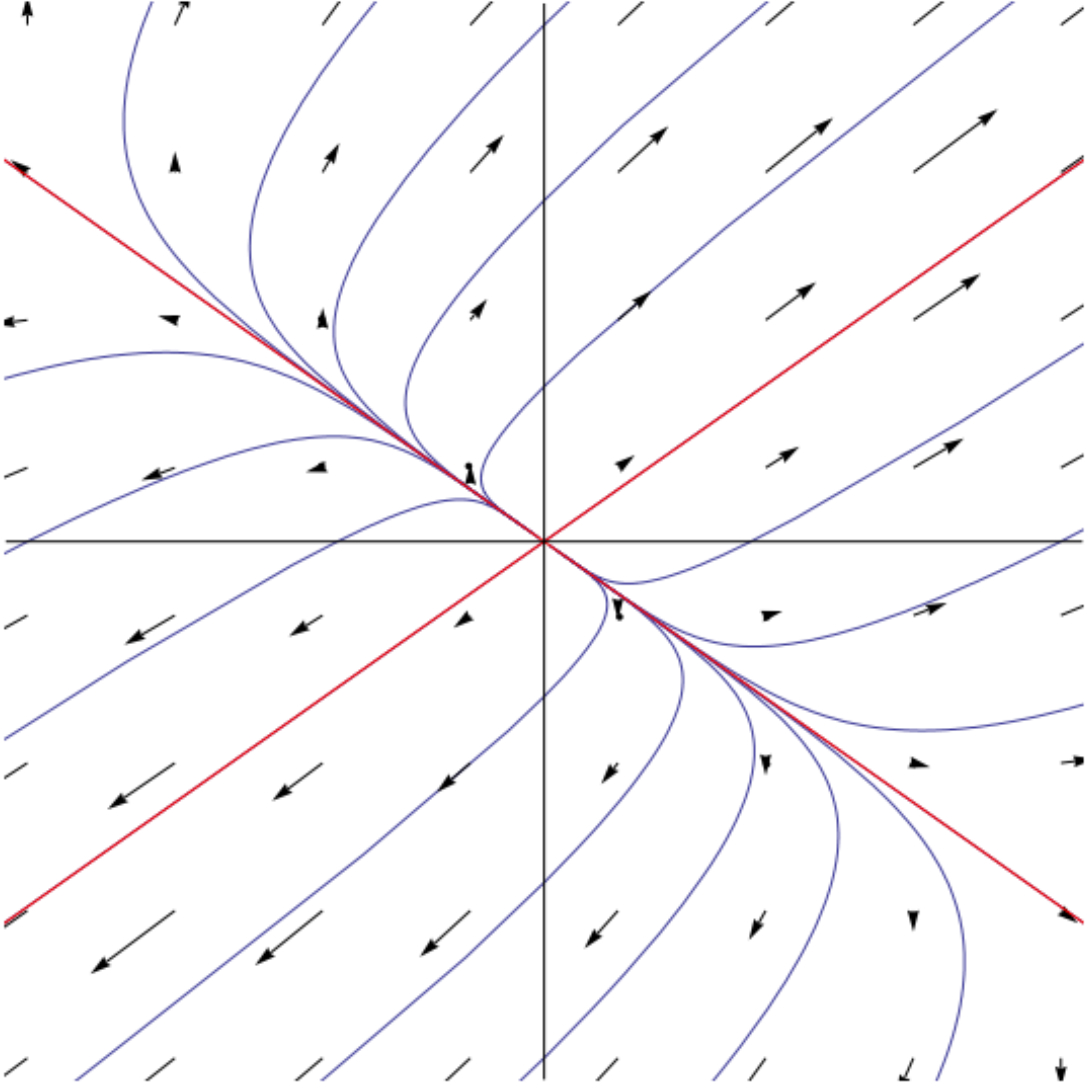
\includegraphics[width=0.8\linewidth]{../ExtFiles/planarRealDiaga.png}
            \caption{$\lambda_1,\lambda_2>0$.}
            \label{fig:planarRealDiaga}
        \end{subfigure}
        \begin{subfigure}[b]{0.32\linewidth}
            \centering
            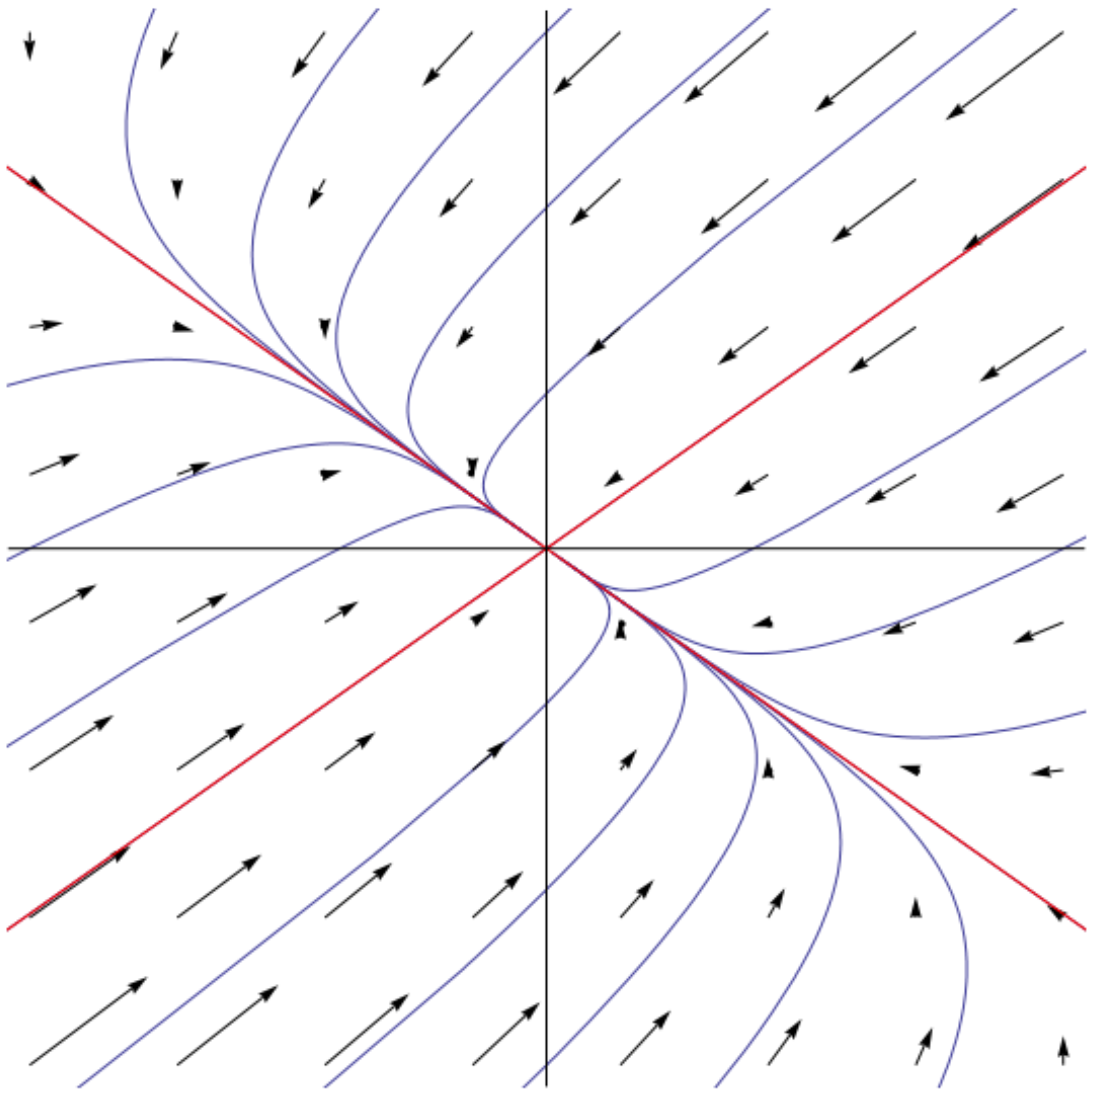
\includegraphics[width=0.8\linewidth]{../ExtFiles/planarRealDiagb.png}
            \caption{$\lambda_1,\lambda_2<0$.}
            \label{fig:planarRealDiagb}
        \end{subfigure}
        \begin{subfigure}[b]{0.32\linewidth}
            \centering
            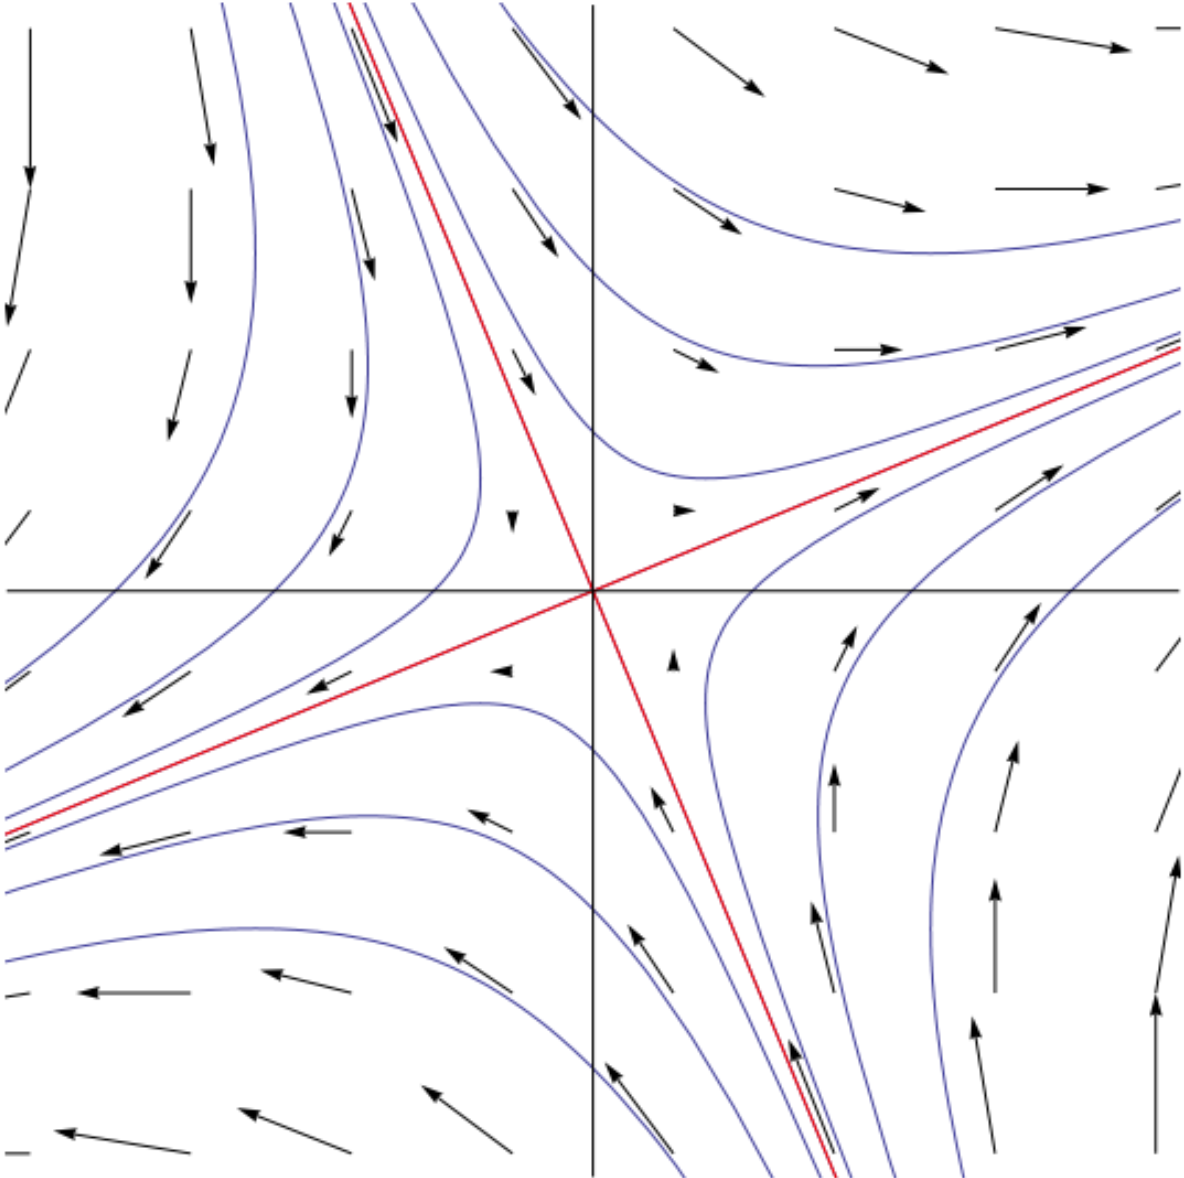
\includegraphics[width=0.8\linewidth]{../ExtFiles/planarRealDiagc.png}
            \caption{$\lambda_1<0<\lambda_2$ (WLOG).}
            \label{fig:planarRealDiagc}
        \end{subfigure}
        \caption{Phase diagrams for a diagonalizable planar system with real eigenvalues.}
        \label{fig:planarRealDiag}
    \end{figure}
    \begin{itemize}
        \item Suppose $\lambda_1,\lambda_2\in\R$ have corresponding linearly independent eigenvectors $v_1,v_2$.
        \item If we choose $v_1,v_2$ to be our basis, then
        \begin{equation*}
            \e[tA] = Q
            \begin{pmatrix}
                \e[t\lambda_1] & 0\\
                0 & \e[t\lambda_2]\\
            \end{pmatrix}
            Q^{-1}
        \end{equation*}
        where $
            Q =
            \begin{pmatrix}
                v_1 & v_2\\
            \end{pmatrix}
        $.
        \item Thus, as before, the solution may be expressed in the following form, where $z=Q^{-1}x$.
        \begin{equation*}
            y(t) = \e[tA]x
            = \e[\lambda_1t]z^1v_1+\e[\lambda_2t]z^2v_2
        \end{equation*}
        \item Moving forward, it will be convenient to work in the $v_1,v_2$ basis. We divide into three subcases ($\lambda_1,\lambda_2>0$ [Figure \ref{fig:planarRealDiaga}], $\lambda_1,\lambda_2<0$ [Figure \ref{fig:planarRealDiagb}], and WLOG $\lambda_1<0<\lambda_2$ [Figure \ref{fig:planarRealDiagc}]).
        \begin{enumerate}
            \item Notice that
            \begin{equation*}
                \e[\lambda_2t] = \e[(\lambda_2/\lambda_1)(\lambda_1t)]
            \end{equation*}
            i.e., $\e[\lambda_2t]$ is a power of $\e[\lambda_1t]$. Thus, when the signs are the same, we get a power function $v_2=v_1^{\lambda_2/\lambda_1}$.
            \begin{itemize}
                \item Both subspaces $v_1,v_2$ are unstable here.
            \end{itemize}
            \item If $\lambda_1,\lambda_2<0$, then we have the same trajectories, but they're all attracted to the origin instead of repelled.
            \begin{itemize}
                \item Both subspaces $v_1,v_2$ are stable here.
            \end{itemize}
            \item When both eigenvalues have different signs, we are considering power functions of a negative power.
            \begin{itemize}
                \item The stable subspace is $v_2$ and the unstable subspace is $v_1$ here.
            \end{itemize}
        \end{enumerate}
    \end{itemize}
    \item Case 3: $A$ has real eigenvalues and \emph{is not} diagonalizable.
    \begin{figure}[h!]
        \centering
        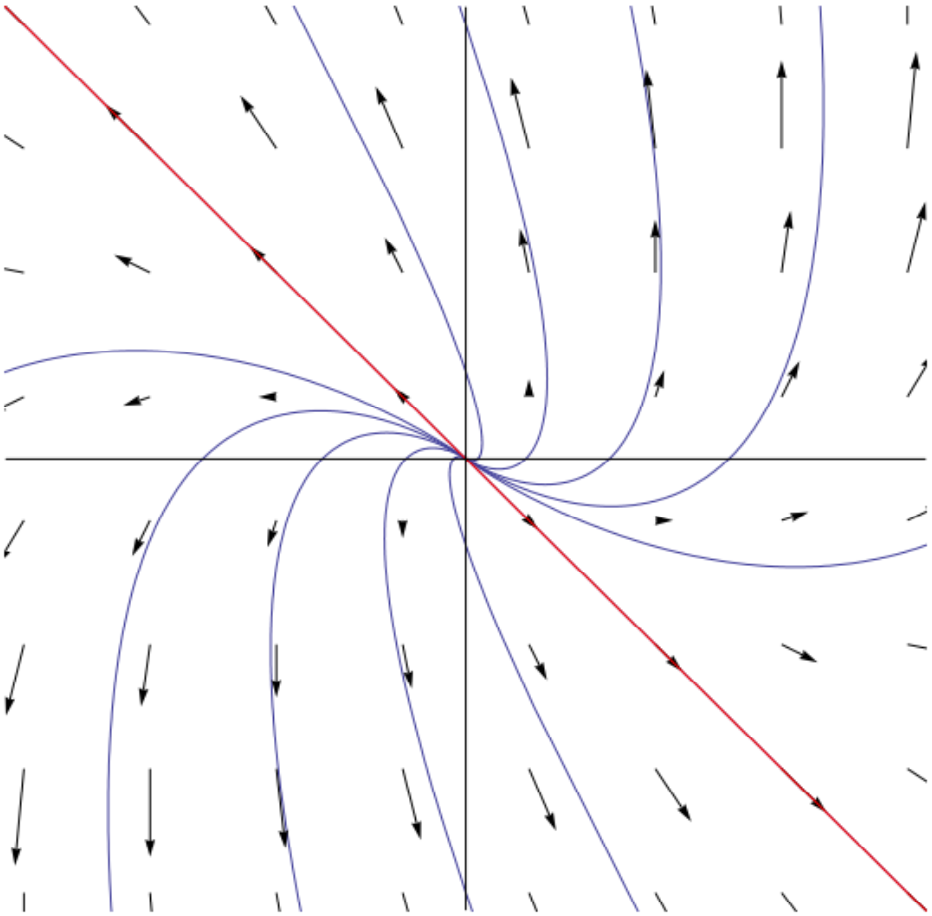
\includegraphics[width=0.256\linewidth]{../ExtFiles/planarRealNon.png}
        \caption{Phase diagrams for a nondiagonalizable planar system with real eigenvalues.}
        \label{fig:planarRealNon}
    \end{figure}
    \begin{itemize}
        \item In this case, the matrix exponential is given by
        \begin{equation*}
            \e[tA] = Q
            \begin{pmatrix}
                \e[t\lambda] & t\e[t\lambda]\\
                0 & \e[t\lambda]\\
            \end{pmatrix}
            Q^{-1}
        \end{equation*}
        \item The solution is given by
        \begin{equation*}
            \e[tA]x = (z^1\e[t\lambda]+z^2t\e[t\lambda])v+z^2\e[t\lambda]u
        \end{equation*}
        where $Q^{-1}x=z$ again.
        \item In graphing, note that here we have (a distorted version of) the form $y=x\pm x\log x$:
        \begin{align*}
            y &= (z^1\e[t\lambda]+z^2t\e[t\lambda])\hat{\imath}+z^2\e[t\lambda]\hat{\jmath}
            \intertext{Define $x:=\e[t\lambda]$. Then $t=\lambda^{-1}\ln x$. Substituting, we have}
            &= (z^1x+z^2(\lambda^{-1}\ln x)x)\hat{\imath}+z^2x\hat{\jmath}\\
            &= (z^1x+z^2\lambda^{-1}x\ln x)\hat{\imath}+z^2x\hat{\jmath}
        \end{align*}
        \item When $\lambda>0$, the whole space is unstable. Thus, the phase diagram is tangent to the origin.
        \item When $\lambda<0$, the trajectories take the same form but this time are attracted to zero. In this case, the whole space is stable.
    \end{itemize}
    \item We can take $x_1$ to $x_2$ iff they are in the same orbit. Conclusion: Orbits never cross.
    \item Takeaway: You should be able to compute the eigenvalues and eigenvectors and sketch these graphs.
    \item Shao will post lecture notes after today's lecture!
    \item Next lecture: The final explicitly solveable case, which is the driven harmonic oscillator.
\end{itemize}




\end{document}